%
Even though the model without the Boussinesq approximation is more consistent, it comes at a price of increased computation time.
This is shown in \cref{fig:perfB}
%
\begin{figure}[htbp]
    \centering
    \begin{subfigure}[h]{0.45\textwidth}
        \centering
        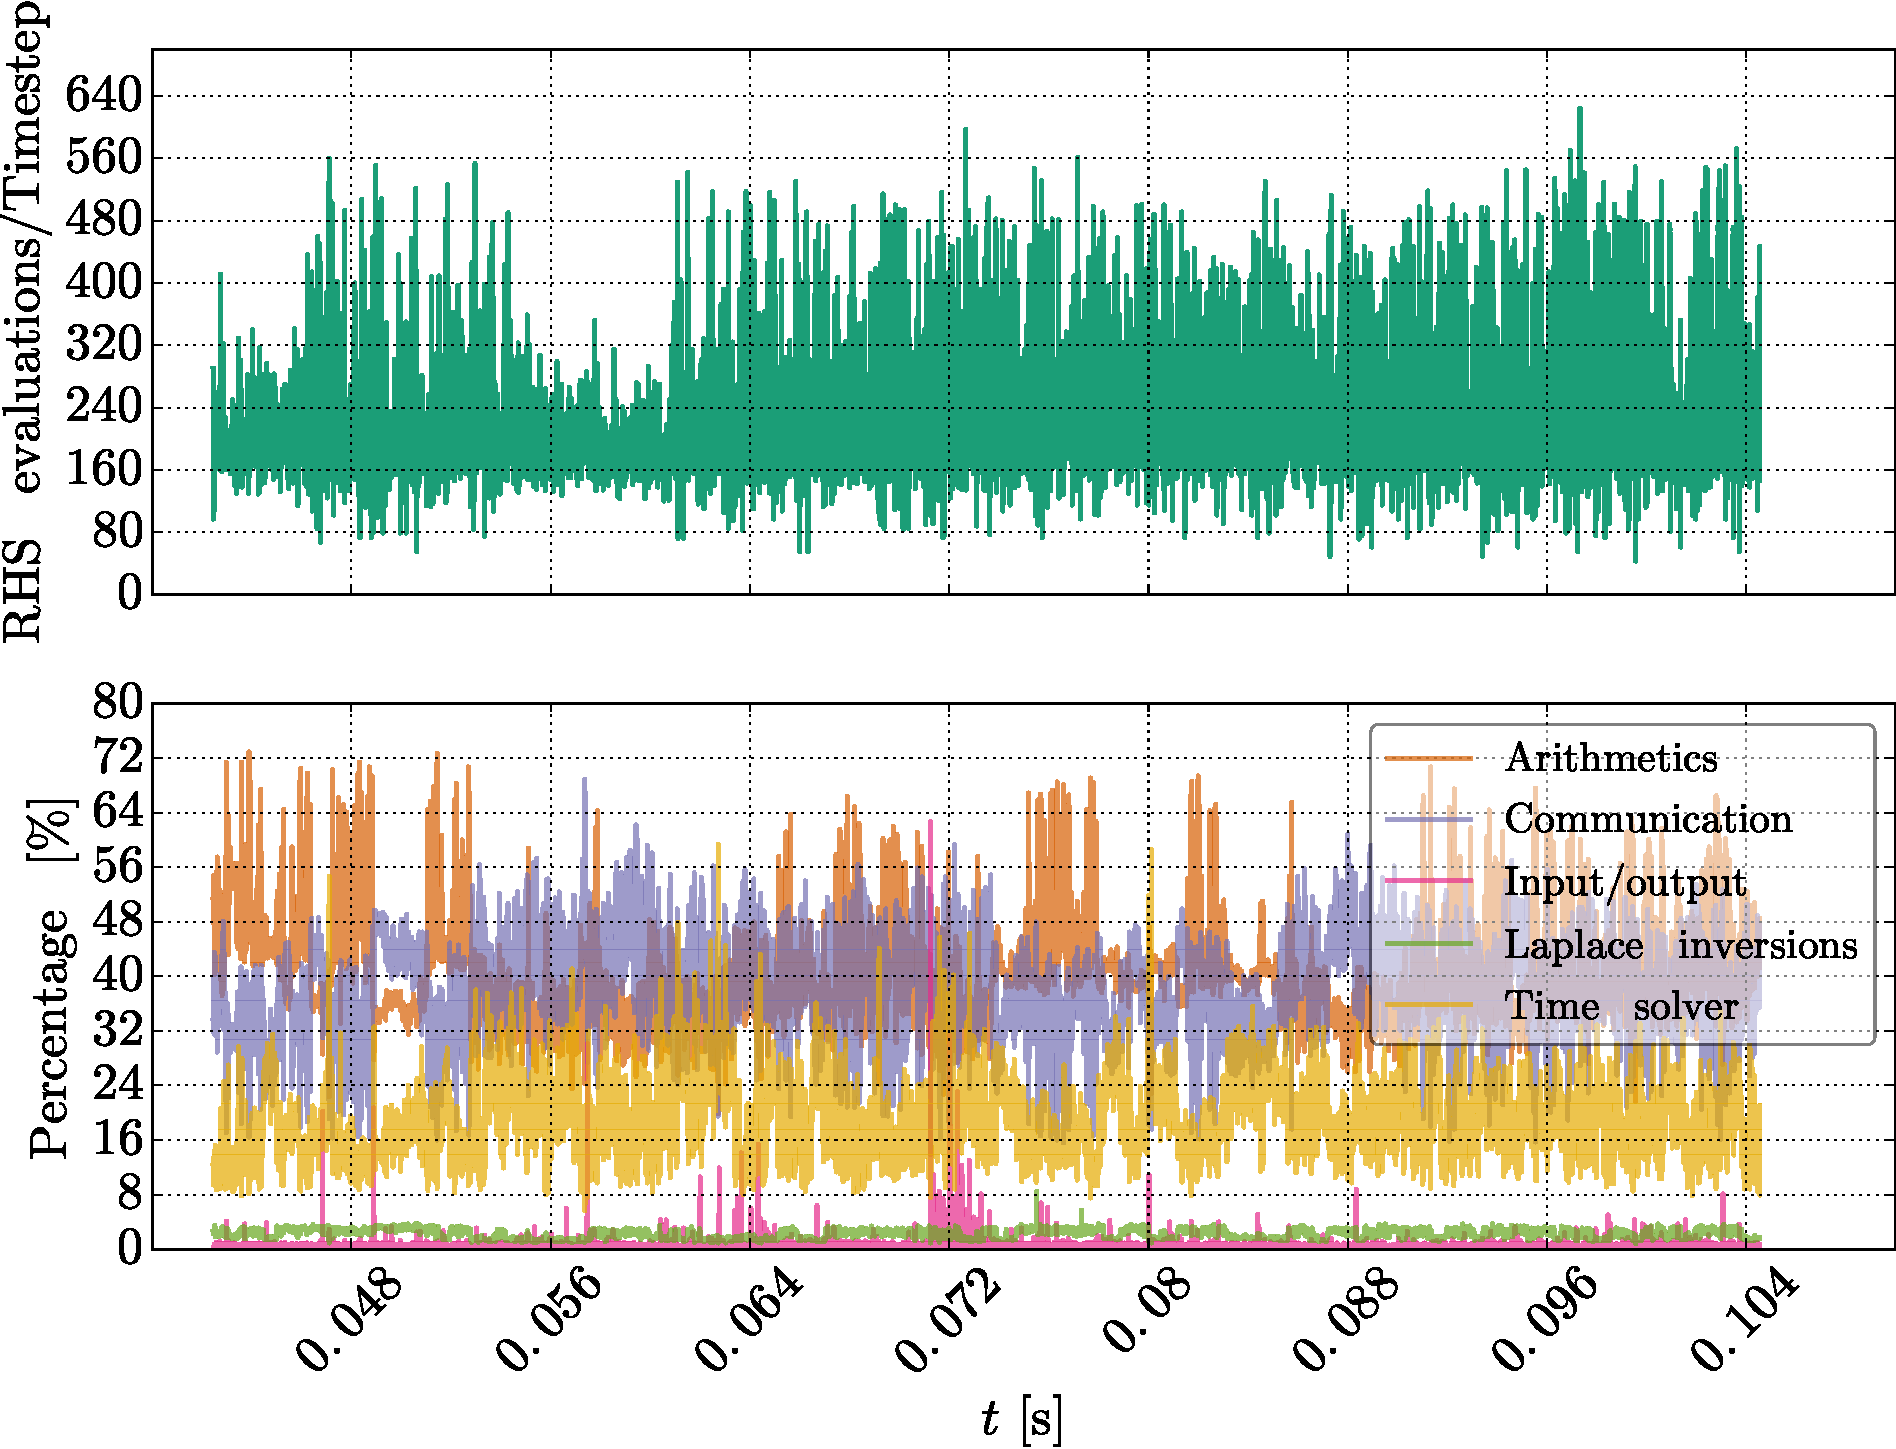
\includegraphics[width=1.0\textwidth]{fig/results/compareBouss/performance004B}
        \caption{$B=0.04\T$}
        \label{fig:perf004B}
    \end{subfigure}%
    \hfill
    \begin{subfigure}[h]{0.45\textwidth}
        \centering
        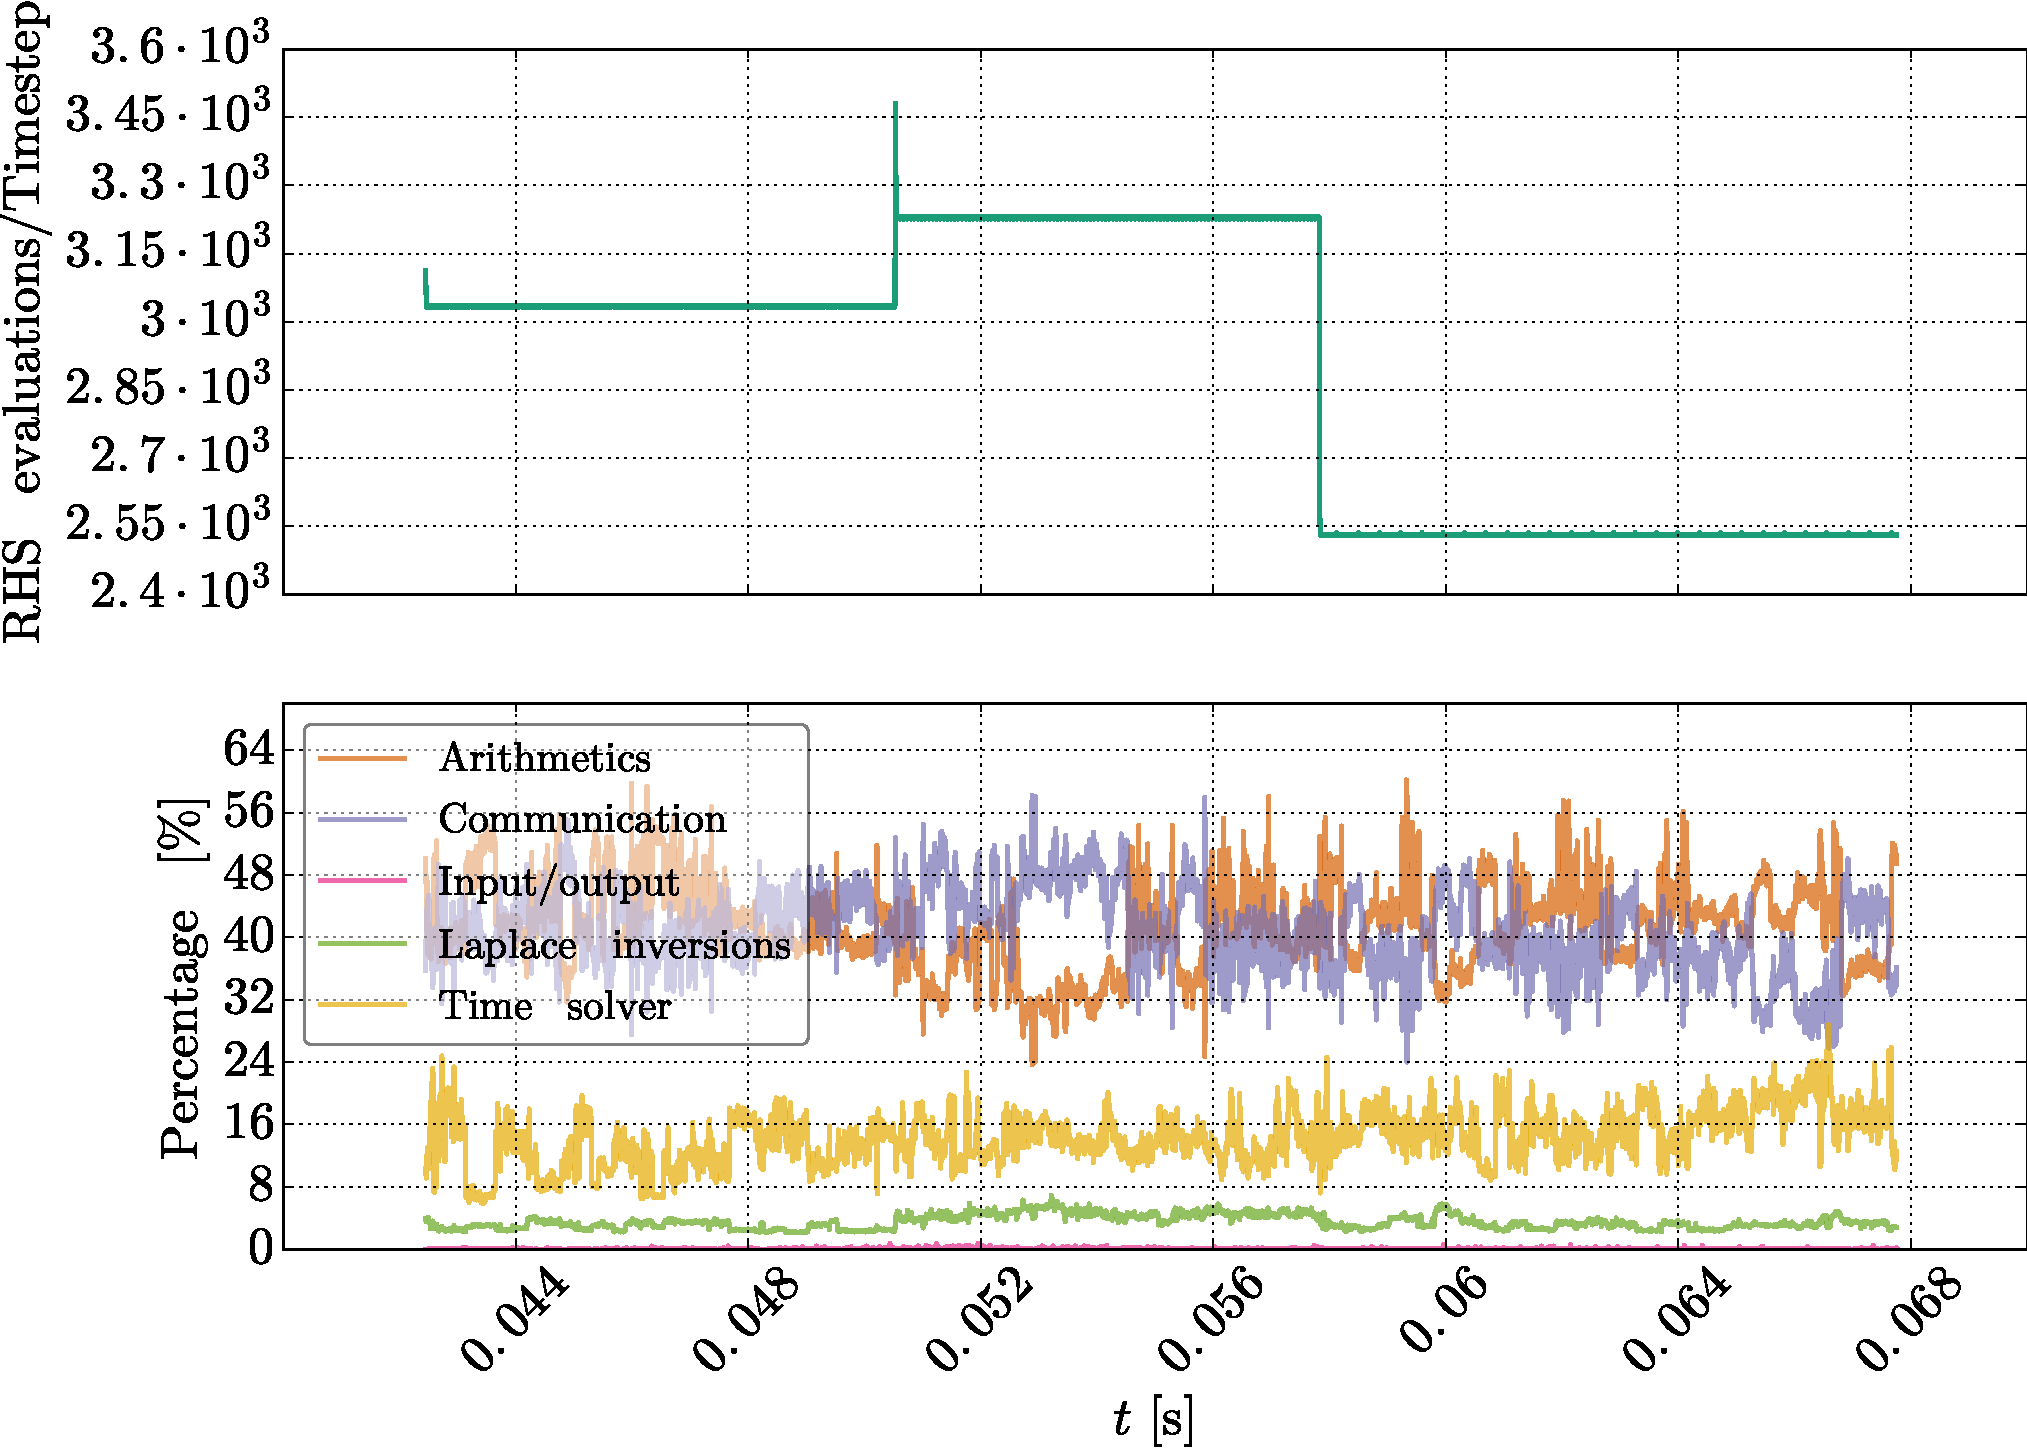
\includegraphics[width=1.0\textwidth]{fig/results/performance/performance004}
        \caption{$B=0.04\T$}
        \label{fig:perf004}
    \end{subfigure}%
    \\
    \begin{subfigure}[h]{0.45\textwidth}
        \centering
        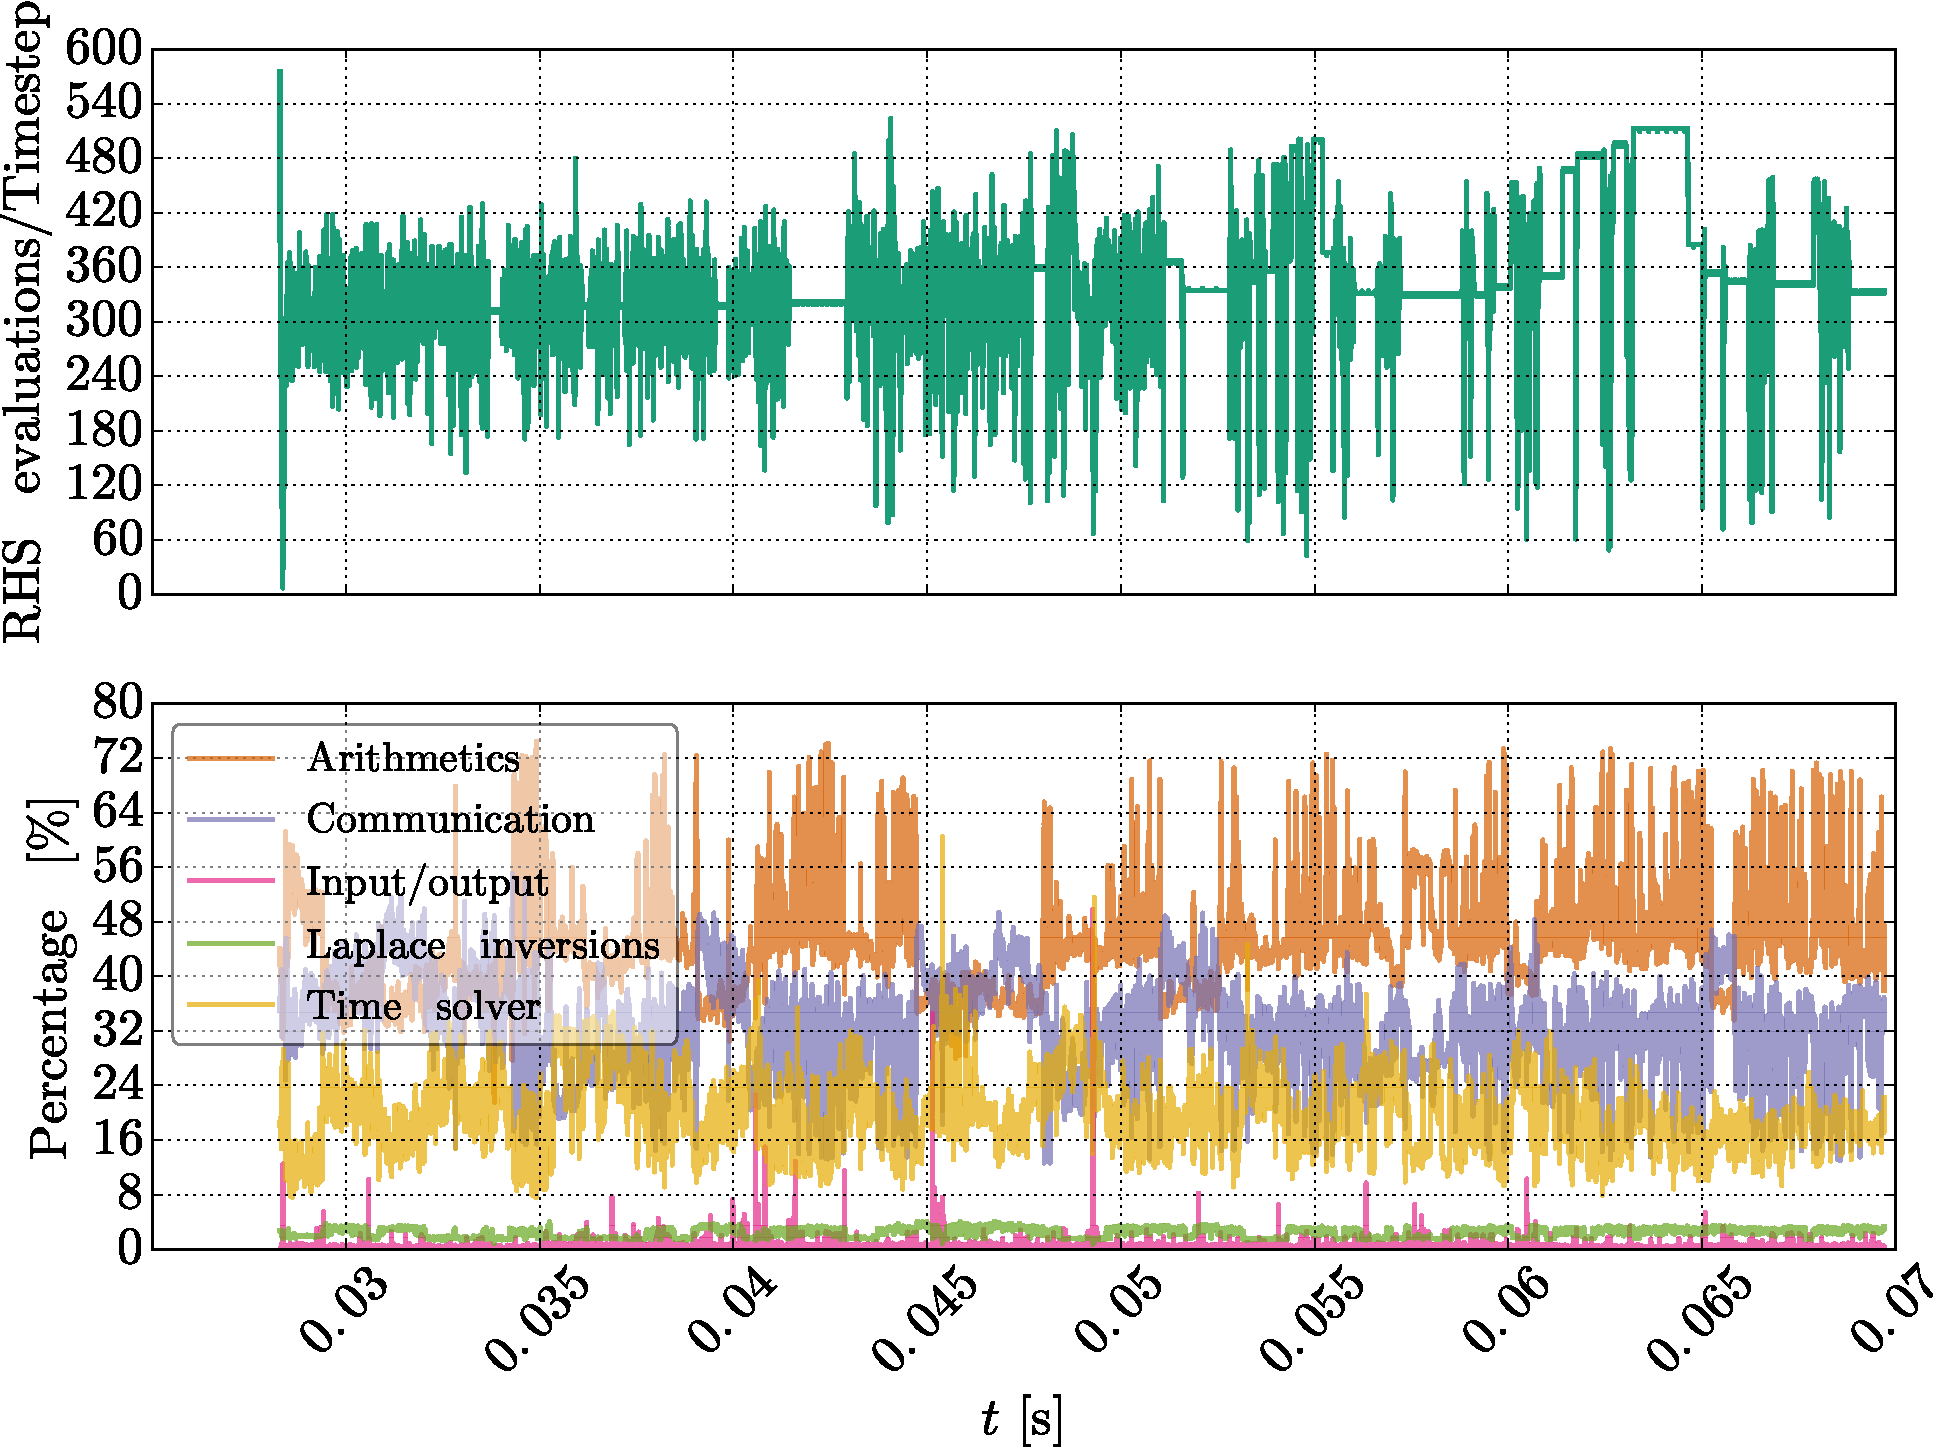
\includegraphics[width=1.0\textwidth]{fig/results/compareBouss/performance006B}
        \caption{$B=0.06\T$}
        \label{fig:perf006B}
    \end{subfigure}
    \hfill
    \begin{subfigure}[h]{0.45\textwidth}
        \centering
        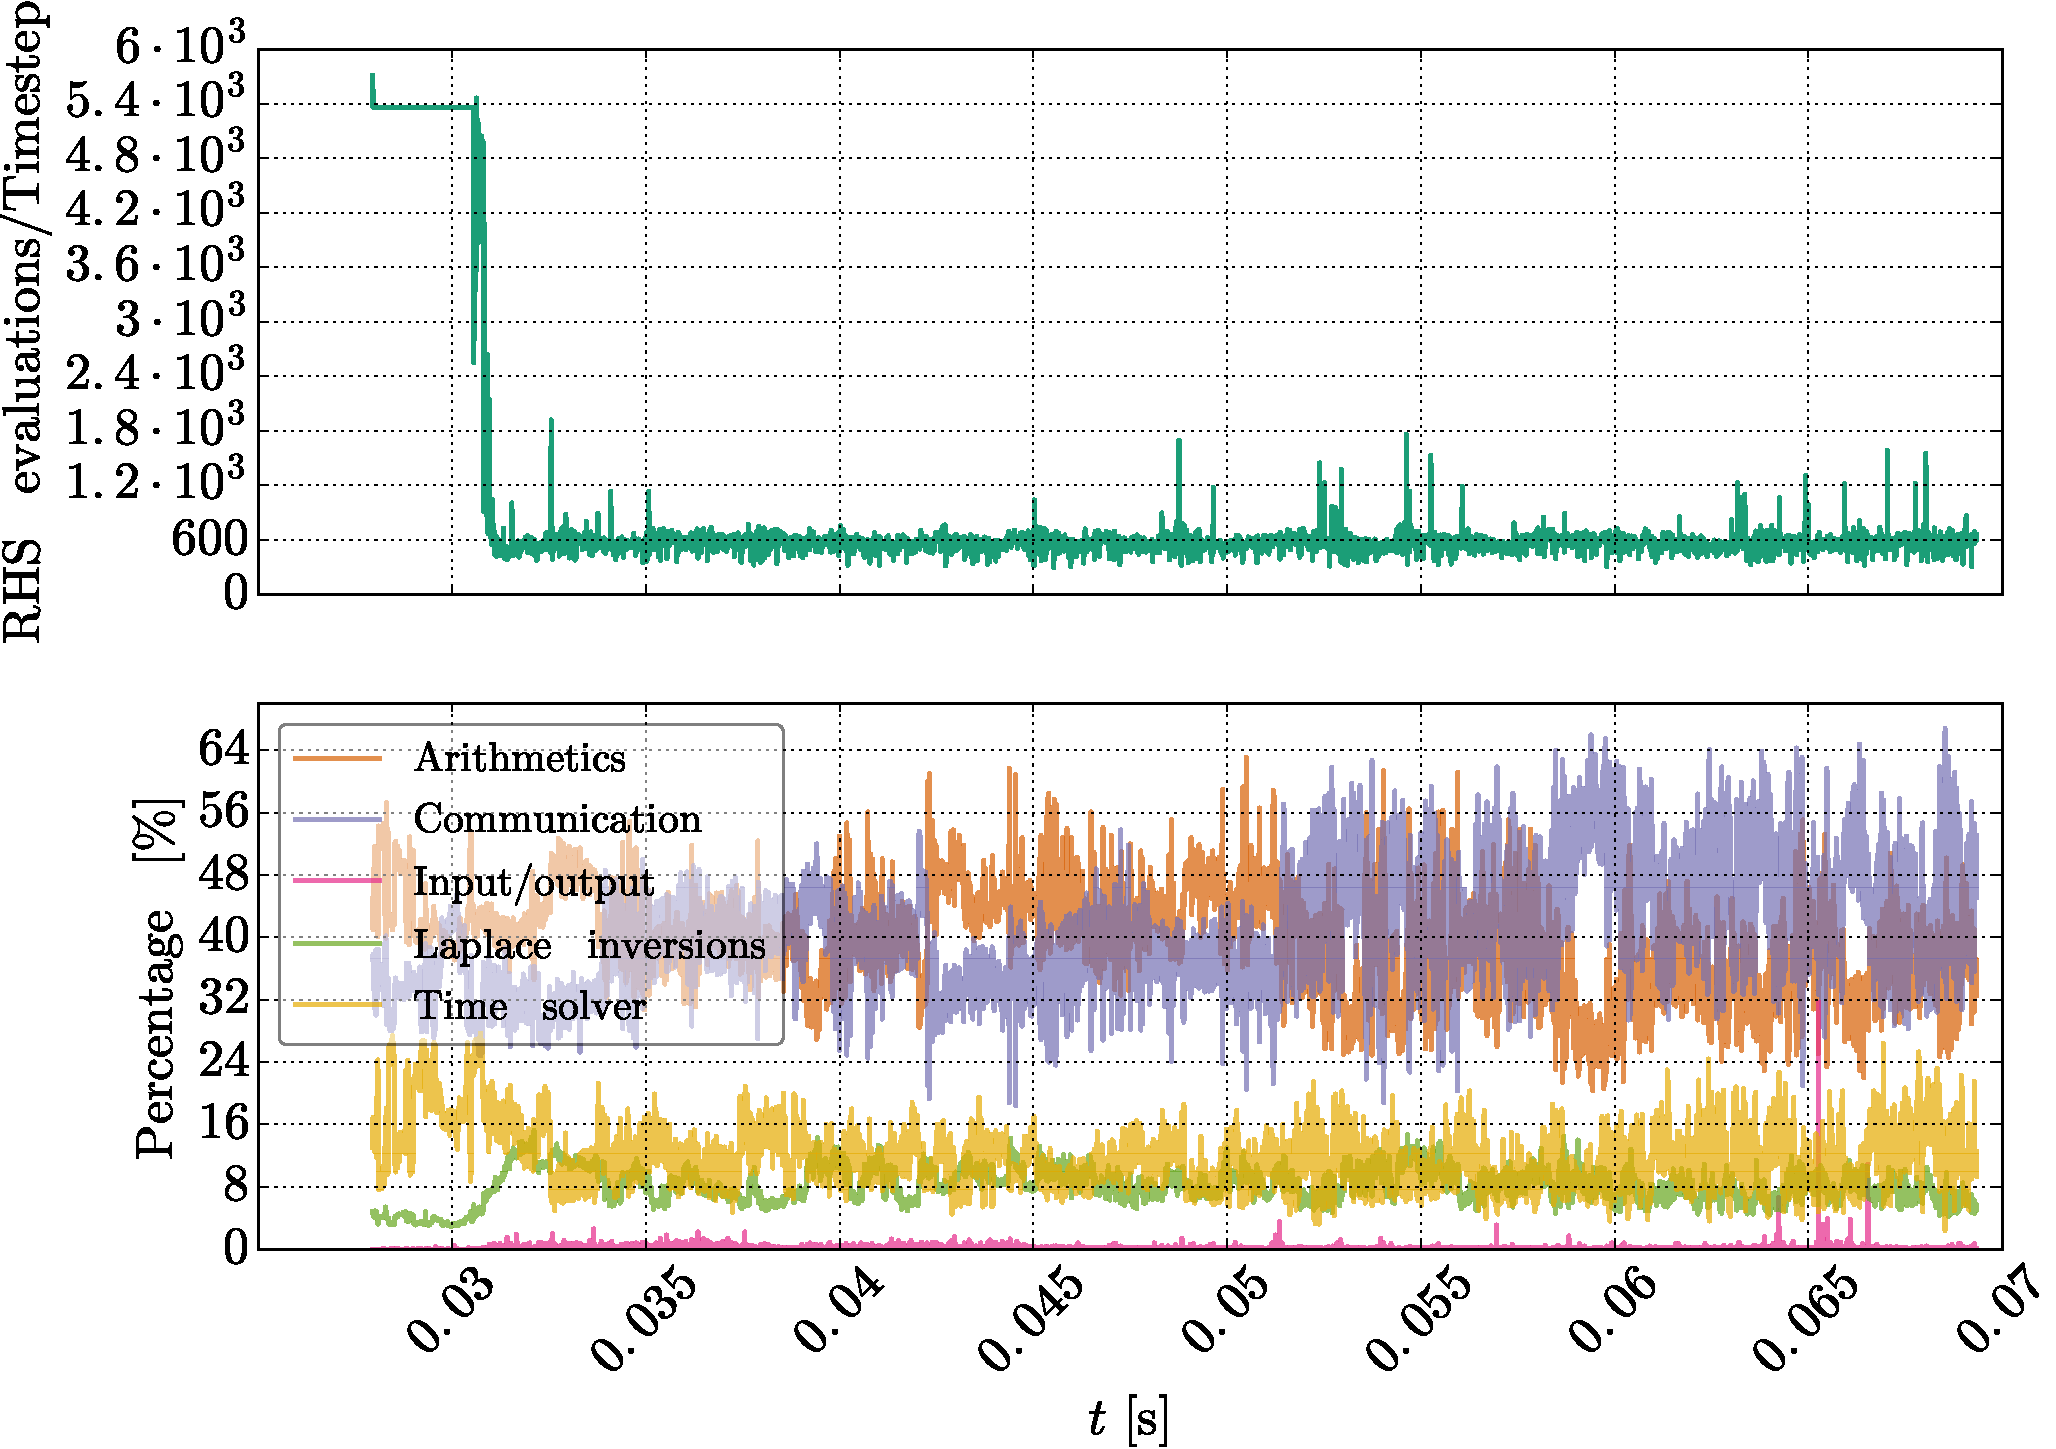
\includegraphics[width=1.0\textwidth]{fig/results/performance/performance006}
        \caption{$B=0.06\T$}
        \label{fig:perf006}
    \end{subfigure}
    \\
    \begin{subfigure}[h]{0.45\textwidth}
        \centering
        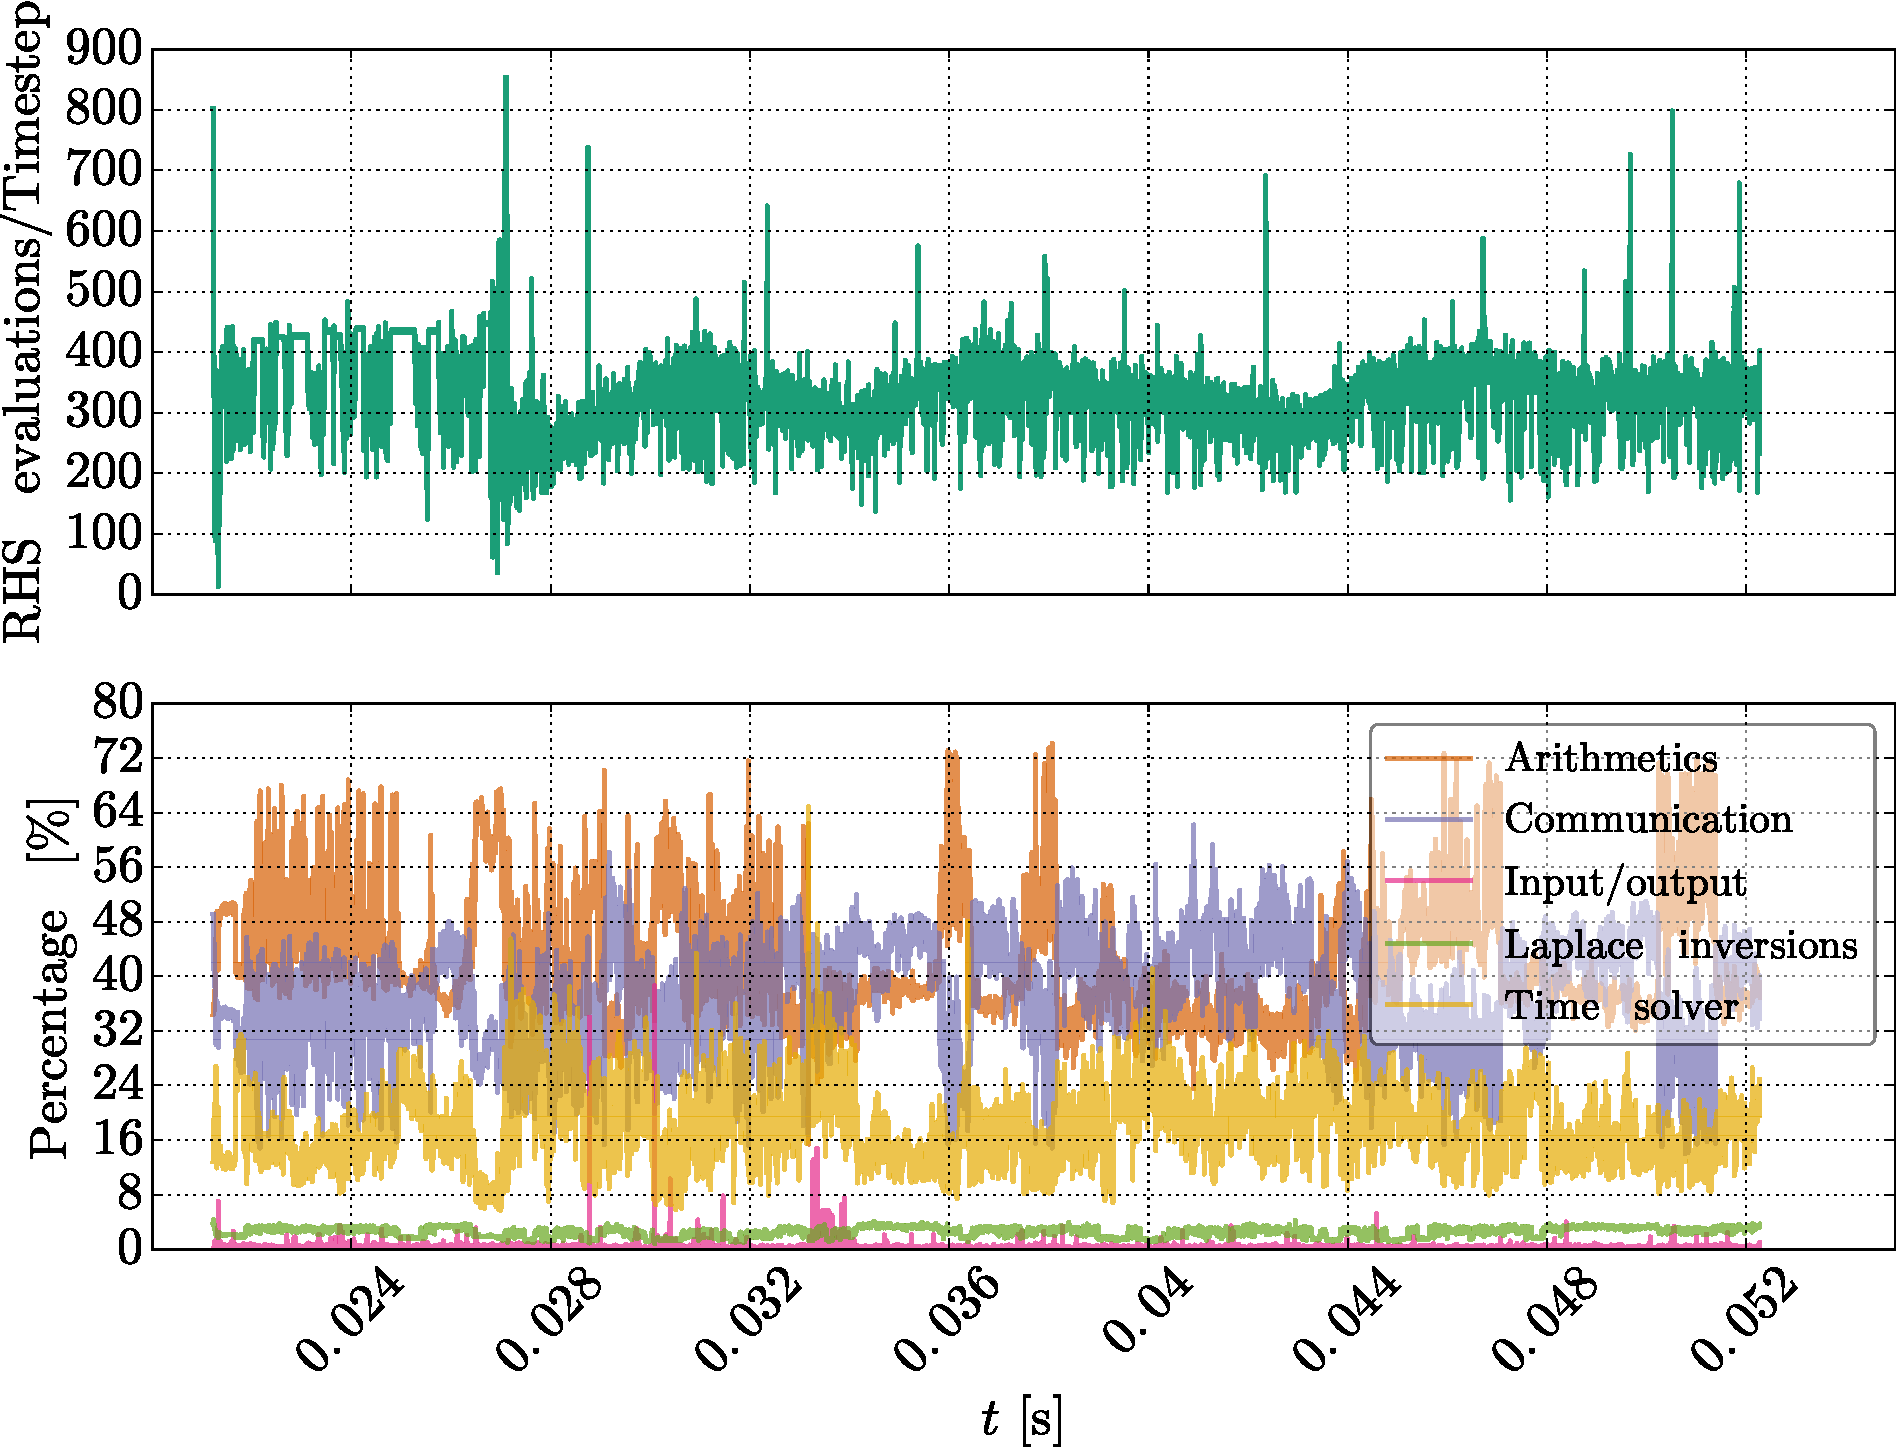
\includegraphics[width=1.0\textwidth]{fig/results/compareBouss/performance008B}
        \caption{$B=0.08\T$}
        \label{fig:perf008B}
    \end{subfigure}
    \hfill
    \begin{subfigure}[h]{0.45\textwidth}
        \centering
        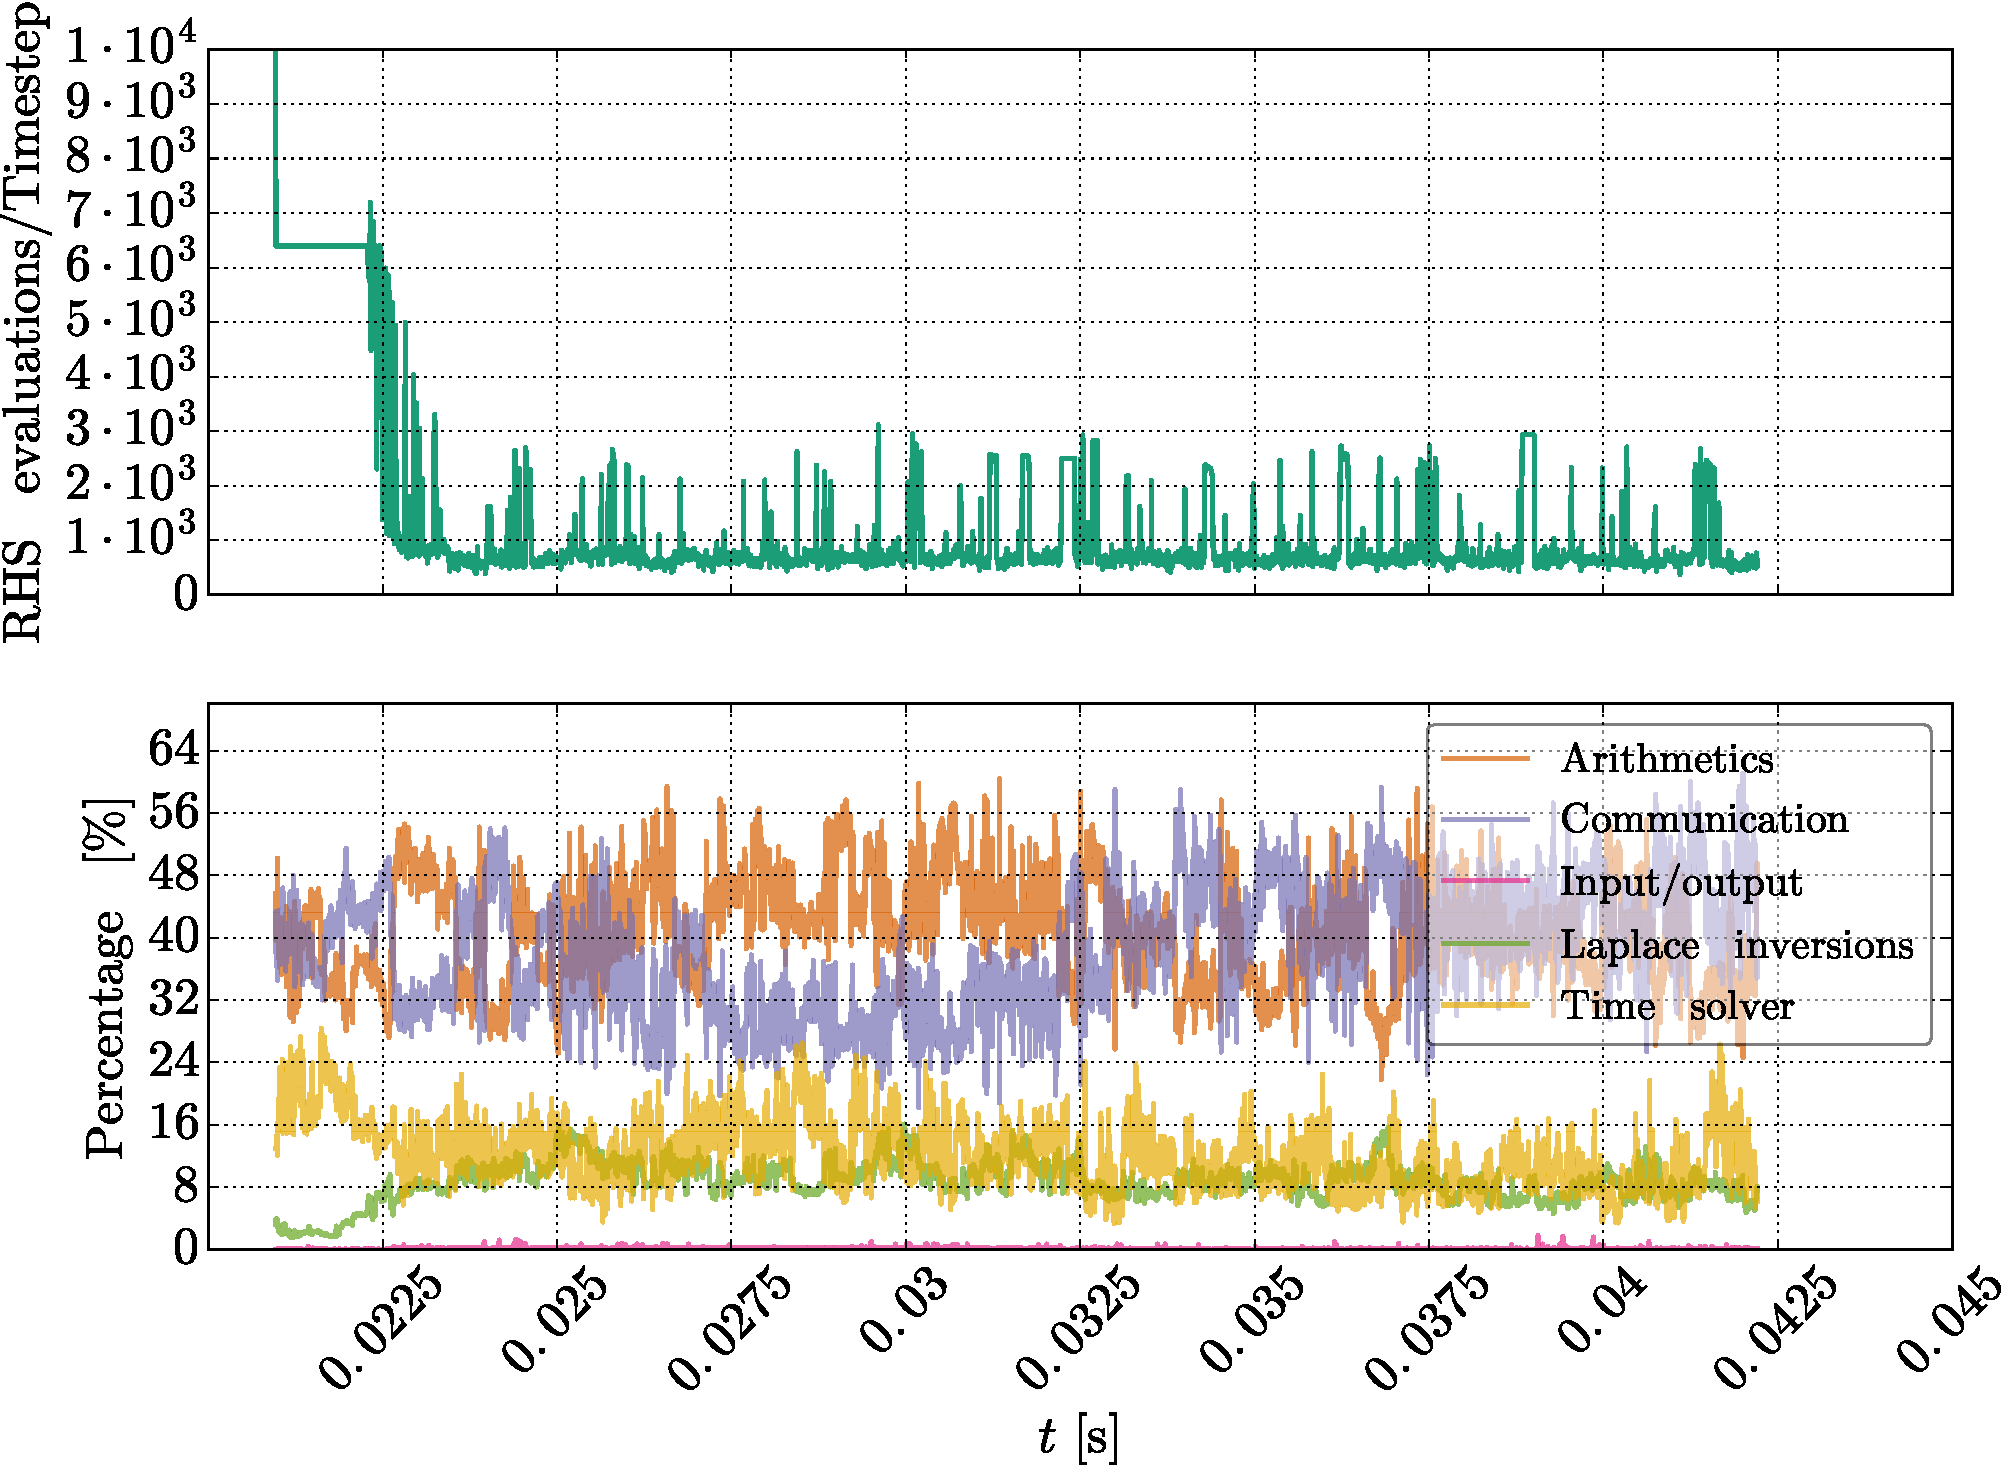
\includegraphics[width=1.0\textwidth]{fig/results/performance/performance008}
        \caption{$B=0.08\T$}
        \label{fig:perf008}
    \end{subfigure}
    \caption{Performance of the code.
        \cref{fig:perf004B,fig:perf006B,fig:perf008B} uses the Boussinesq approximation, whereas \cref{fig:perf004,fig:perf006,fig:perf008} does not.}
    \label{fig:perfB}
\end{figure}
%
Before the added perturbation, the simulations using the Boussinesq approximation uses around $100$ iterations per time step, whilst the non-Boussinesq model uses between $4000 - 12000$ iterations per time step.

In the non-Boussinesq case, the iteration count is almost constant, and higher than in the saturated turbulence case.

Most of the simulation time is done when communicating between processors and doing arithmetic operations on the fields for both models.
The time used in the external time solver (\texttt{cvode}) is always less than this.
In the Boussinesq case there is a significant increase of time used in both the communication process and the Laplace inversion (where the potential is solved from the vorticity).
This can be explained by the extra communication and inversion needed in the iterative Naulin solver, which uses between $3-10$ iteration per time step in the saturated turbulent phase.
